\documentclass[12pt]{article}
\usepackage[margin=.8in]{geometry}
\usepackage{graphicx,hyperref,parskip}
\hypersetup{colorlinks,
    citecolor=black,
    filecolor=black,
    linkcolor=black,
    urlcolor=black
}

\newcommand{\HRule}{\rule{\linewidth}{0.5mm}}


\begin{document}
\newpage

\begin{titlepage}
\begin{center}
\textsc{\LARGE }\\[1.5cm]
\textsc{\Large Proposal 2}\\[0.5cm]

\HRule \\[0.4cm]
{\huge \bfseries Ripieno}\\
\HRule \\[1.5cm]

Tyler \textsc{Babaran}\\
Kevin \textsc{Carruthers}\\
Lara \textsc{Janecka}\\
Nik \textsc{Klassen}\\
Josh \textsc{Netterfield}\\
Eric \textsc{Pemberton}\\

\vfill
{\large \today}
\end{center}

Instructor: Christine Horton
\end{titlepage}

\tableofcontents
\newpage

\section{Ripieno}
\subsection{Introduction (Kevin)}
Ripieno is an upcoming music notation app brought to you by the Ripienist team.

Our team is developing Ripieno to fill a specific gap in the world of music notation: the missing ability to easily create and share sheet music. Any composer who wishes to share his work without Ripieno is forced to spend time scanning and compiling his written composition, transform that scan into a viewable file, and send that file to anyone who may be interested.

With Ripieno, all that composer would need to do is click the ``share'' button.

This product is useful for several reasons:
\begin{itemize}
\item teachers can use Ripieno to more easily teach their students; students can use Ripieno to learn about music composition
\item any composer, hobbyist or professional, can easily share their work
\item groups interested in composing a piece can work together
\end{itemize}

Ripieno is marketed towards local musicians, both hobbyists and professionals. In its simplest terms, Ripieno is of use to any individual with the desire to create or share sheet music; this can include music teachers, music enthusiasts, or even professional musicians.

More specifically, Ripieno is marketed towards Waterloo and Wilfred-Laurier students: whether they are majoring in music or are simply interested in it, they can use Ripieno to explore their musical instincts.

\subsection{Proposed Project (Josh)}
Ripieno will be a high-quality, easy-to-use music score-writer with an emphasis on collaboration and mobility. In particular, it is a web application as well as a native app for iPads, Macs, and PCs. Songs created on any platform are automatically synced to all other platforms and can be shared with any number of other users.

Professional sheet music notation software (``score-writers'') currently on the market have a high barrier to entry both in terms of cost and usability, and sharing sheet music often involves printing it out due to incompatibilities in formats, even between versions of the same software. In addition, no professional sheet music engraver also provides mobile editing.

Students taking courses in composition and arranging can use the collaboration feature of Ripieno to submit assignments. Instructors can then make suggestions directly on the sheet music without printing. In addition, semi-professional musicians with a large library of music can use Ripieno to cheaply and efficiently manage and add to their repertoire.

\subsection{Costs and Requirements (Eric)}
The costs of developing this project will come in three stages; product development, marketing and maintenance.

\begin{itemize}
\item {\bf Product Development}: the costs associated with developing Ripieno include the purchase of all required technologies to build the software, as well as the cost to hire software developers and Quality Assurance team members.
\item {\bf Marketing}: The costs for marketing the product will include online advertising, product demoes for interested parties, and brand promotion.
\item {\bf Maintenance}: Maintenance costs will include customer support, addressing bugs that clients discover, and developing fixes.
\end{itemize}

\subsection{Research (Nik)}
The age of digitization has affected almost every field, music included. Music stores are no longer able to maintain the market they once had due to the sheer amount of merchandise available online. The Joseph Patelson Music House in New York City is just one example of the many music stores that have closed due a lack of customers [1].  Music students are now performing and composing their music using digital media. There are many tablet applications available to display music while performing. These applications allow users to download content from various music collections on the web [2]. However, changes to the ways music is created are unable to proceed if composers do not have easy ways to create their sheet music digitally.

Composers working with publishing houses have access to proprietary software such as Finale, but with a price tag easily ranging beyond \$600, this software is inaccessible for educators and students [3]. Students are far more unwilling to take up a hobby if experimenting with it is expensive. In addition to cost, students wish to share their creative output with friends and get input from those who are more experienced.  Students say they find a hobby or new field of study much more fulfilling if they feel that they are making progress---and even more importantly, doing it properly. Our music notation app aims to make music more easy to share, to give the collective knowledge of the music community to our users.

\subsection{Assets (Eric)}
To complete this project the following assets are available to the Ripieno team:
\begin{itemize}
\item The use of Javascript in the product is supported with extensive online documentation including design strategies for ``Node.js''. This will cut down on the amount of time required to develop the product.
\item Music theory and notation is covered through a written notation book detailing every intricacy involved in rendering sheet music. This resource will allow Ripieno to create in-depth coverage of all music notation styles needed by users.
\end{itemize}

\subsection{Progress So Far (Kevin/Lara)}
\subsubsection{Accomplishments to Date}
After a few days of deliberation, the Ripienists had a detailed design plan outlined. Due to good group cohesion, a design was decided upon very quickly with full group consensus. Coming into the project, Josh already had a design in mind---thus accelerating the project development. There was a short discussion over which testing framework between Tyler and Eric during the third meeting. The design planned was finished after Nik and Josh finally agreed on the correct front-end framework to use. Overall, the team arrived an a collectively accepted design to-be-implemented.

Currently, the team is just wrapping up the testing for a basic beta version of the final product. Rudimentary functionality has been achieved and testing has returned few bugs, all of which easily fixed. Kevin has just finished some market research and is currently drafting some changes to the front-end interface to make it more appealing to our potential clients.

\subsubsection{Future Goals}
Going forward, the Ripienists will be implementing the front-end interface changes as drafted by Kevin. Furthermore, there is a large list of features to be included in the next release:
\begin{itemize}
\item multi-staffed instruments
\item viewing multiple instrument lines simultaneously
\item collaborative chat
\item auto-import from tools such as Finale
\end{itemize}
and several others.

The features listed above will definitely be included in the next release, as well as fixes for any bugs our Quality Assurance team discovers in the meantime and any other features as time permits.

\begin{figure}[ht]
\centering
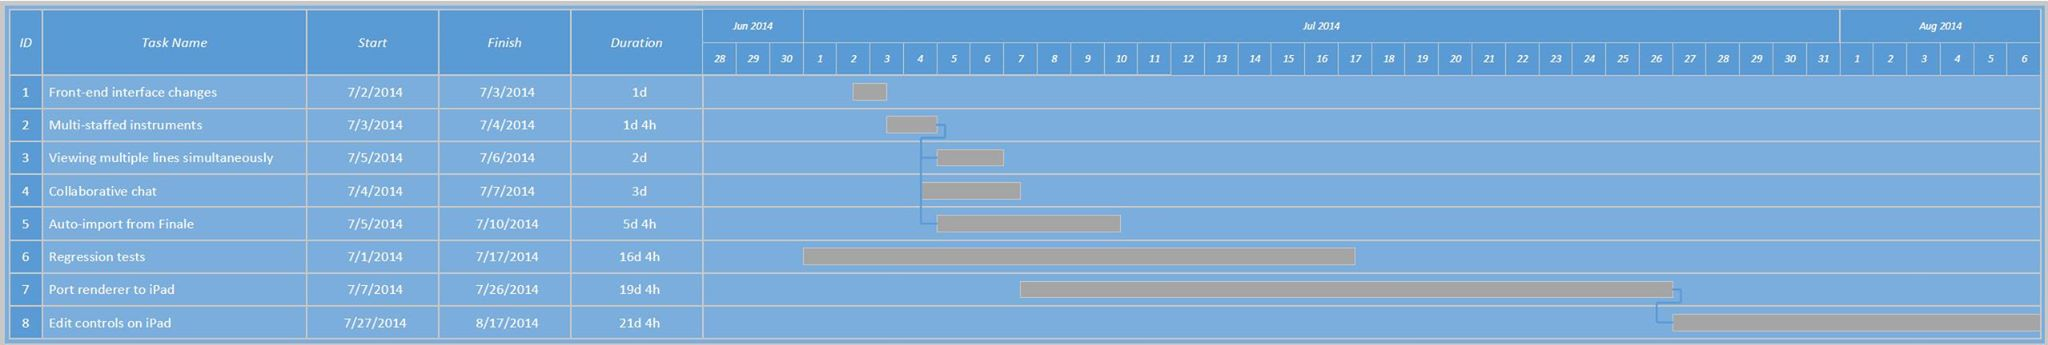
\includegraphics[width=\textwidth]{gannt.jpg}
\caption{Gannt Chart}
\end{figure}

\subsection{Team Structure (Tyler)}
The Ripienist team is structured as follows:
\begin{itemize}
\item Josh Netterfield is the creative genius behind Ripieno, and will be our lead software developer thanks to his experience at Khan Academy.
\item Nik Klassen is our assistant developer with four years of experience developing teaching tools at Desire 2 Learn.
\item Lara Janecka will be operating as the project leader due to her experience in a managerial position at Auvik Networks Inc.
\item Kevin Carruthers has been designated chief of marketing. As a renowned spokesperson for Staples Business Depot, his experience will be invaluable.
\item Eric Pemberton and Tyler Babaran are specialists in Software Quality Assurance and testing, with over five years of experience each at Blue Coat Systems and Unitron Canada respectively.
\end{itemize}

\subsection{Conclusion (Lara)}
Ripieno fills a much needed niche in Waterloo. The music departments within the University of Waterloo and Wilfred-Laurier University provide a large market of young musicians who are already share large portions of their lives via the Internet. Musicians are often very passionate toward their craft and need a way to easily share this with others. Ripieno allows musicians to share and collaborate with the same ease as one might share a project proposal via Google Docs. Based on the above results, the Ripienist team would like to proceed with the development phase of the project.
\newpage

\section{Sources}
\begin{enumerate}
\item http://www.nytimes.com/2009/04/13/arts/music/13pate.html?\_r=0
\item http://www.theatlantic.com/technology/archive/2011/08/musicians-embrace-the-ipad-leave-sheet-music-at-home/243726/
\item https://store.makemusic.com/Store/default.aspx?tab=notation
\end{enumerate}

\end{document}
